%
% latex-sample.tex
%
% This LaTeX source file provides a template for a typical research paper.
%

%
% Use the standard article template.
%
\documentclass{article}
\usepackage{graphics} % for pdf, bitmapped graphics files
\usepackage{epsfig} % for postscript graphics files
\usepackage{mathptmx} % assumes new font selection scheme installed
\usepackage{times} % assumes new font selection scheme installed
\usepackage{amsmath} % assumes amsmath package installed
\usepackage{amssymb}  % assumes amsmath package installed
\usepackage{chngpage}
\usepackage{lipsum}
\usepackage{listings}
\usepackage{xcolor}

% The geometry package allows for easy page formatting.
\usepackage{geometry}
\geometry{letterpaper}

% Load up special logo commands.
\usepackage{doc}

% Package for formatting URLs.
\usepackage{url}

% Packages and definitions for graphics files.
\usepackage{graphicx}
\usepackage{epstopdf}
\DeclareGraphicsRule{.tif}{png}{.png}{`convert #1 `dirname #1`/`basename #1 .tif`.png}

\lstset { %
    language=Python,
    backgroundcolor=\color{black!5}, % set backgroundcolor
    basicstyle=\footnotesize,% basic font setting
}

%
% Set the title, author, and date.
%
\title{City Traffic Simulation in Javascript and WebGL}
\author{Aven Bross}
\date{5/7/2015}

%
% The document proper.
%
\begin{document}

% Add the title section.
\maketitle

% Add an abstract.
\abstract{
In this paper I explore a simulation of streetlights and city traffic.  The goal is to create a small section of city with cars passing through that can be manipulated and examined.  Traffic density, where cars are going, and where they enter from will vary.  By examining build up and statistics, the hope is to be able to establish optimum lane layouts and streetlight timings to minimize traffic halting and clogging.
}

% Add various lists on new pages.
%\pagebreak
%\tableofcontents

%\pagebreak
%\listoffigures

%\pagebreak
%\listoftables

% Start the paper on a new page.

%
% Body text.
%

\section{Introduction}

The goal of this project is to create a sandbox system to simulate a subsection of city traffic.  Cars will enter the subsection with a desired destination and progress through the traffic lights and stop signs. By examining where and how traffic builds up under different conditions, I hope to allow optimization of traffic light timing and city layout within the subsection.  The simulation should allow varying where traffic enters, where popular destinations are and the density of traffic. By observing these changing variables over time, optimum timings and layouts can be found to fit traffic pattern changes based on time of day as well.

\section{Model}

The traffic model I have decided on utilizes discrete grid cells for car movement and routing decisions.  Speed and movement will not be appear discrete or jumpy but the underlying system will be "turn-based" in nature to allow for a simple decsion making system and remove the need for collsion detection.

\subsection{City Layout}

The city layout shall be simulated as a grid system.  Each square shall have a value \emph{direction} and a value \emph{empty}.  The \emph{direction} value will be an integer represented cardinal direction indicating whether the given square is a lane going a certain direction, or a null value to represent a piece of an intersection or other non-directioned road.  The \emph{empty} value will simply indicate whether the square is open to be moved into.  Squares may also be subject to street lights, preventing their occupants from moving on until a reasonable value is reached.

\subsection{Cars}

Cars in the simulation will be simple constructions that have a \emph{position} in floating point x,y coordinates, a \emph{direction} as an integer in the same format as above, a floating point \emph{speed} value and a possible \emph{destination} in x,y coordinates.  Upon a move call the car will move in its forward direction unless obstructed or faced with an intersection or turn possibility.\\
For the current simulation, destination pathing was ommitted.  Since it would be a fairly complicated user interface to allow manipulation of popular destinations and  starting points, cars will simply make random decisions as they are faced with movement options.\\
It should also be noted that decisions to move forward are weighted higher, for example as a car moves into the first squuare of an intersection, it has a $\frac{2}{3}$ chance to go forward, with only $\frac{1}{3}$ chance of making a right turn.

\subsection{Simple System}

Here is a diagram for a simple intersection.  Arrows indicate lane direction, grey squares indicate impassable.

\centerline{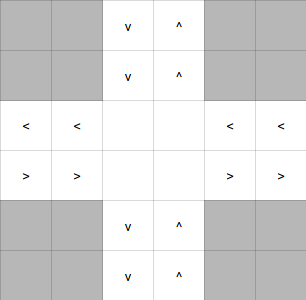
\includegraphics[width=5cm, height=5cm]{city_grid}}

\noindent The algorithm for determining possible decisions for a car is outlined in pseudocode below.  This will be refined and added to for multiple lanes, stop lights, and many other situations.

\begin{adjustwidth}{1.5em}{1.5em}
\begin{lstlisting}
if forwardSquare.empty
    add possibility MOVE_FORWARD
if rightSquare.direction is right
    add possibility TURN_RIGHT
if leftSquare.direction is left
    add possibility TURN_LEFT
else if leftSquare.direction is none
    while leftSquare.direction is none
        set leftSqare to the next left square over
    if leftSquare.direction is left
        add possibility TURN_LEFT
\end{lstlisting}
\end{adjustwidth}

\noindent The car would then look at the possibilities and make a decision based upon its desired \emph{destination}.

\subsection{Movement}

Each car has a speed which will determine speed of movement.  When a car makes a movement decision, they choose a destination square and set it as occupied. Over time they will progress to their destination square and will then not make a further decision until such time that they reach their destination state.  Upon reaching the quarter-way point, they will mark their previous square as empty.  We will assume cars will be maintaining low city speeds and speed will not vary between cars enough to cause collision detection problems with this mehtod.

\subsection{Streetlights}

Stoplights are modeled as separate entities each with an \emph{x,y} position, an integer \emph{state} and three timing variables \emph{redtime}, \emph{yellowtime} and \emph{greentime}.  The \emph{position} denotes the top left corner of the intersection the street light will be managing.  There are six possible \emph{state} values that are cycled through in order: green vertical, yellow vertical, red all, green horizontal, yellow horizontal, red all.  The amount spent in each state is determined by the timing variables above.\\
Streetlights manage traffic by marking squares with which direction movement is allowed.  Cars in turn incorporate this into their logic by checking the square ahead does not have a stoplight car for its current direction

\section{Simulations}

The city map constructed for the simulation was ultimately decided to be a uniform grid pattern.  Each intersection is constructed as per the image below, as a 6 by 6 section of grid cells.  The middle four form the intersection, with a stoplight managing them. Directed lanes enter and exit at the proper sides and impassible squares occupying the corners.\\

\centerline{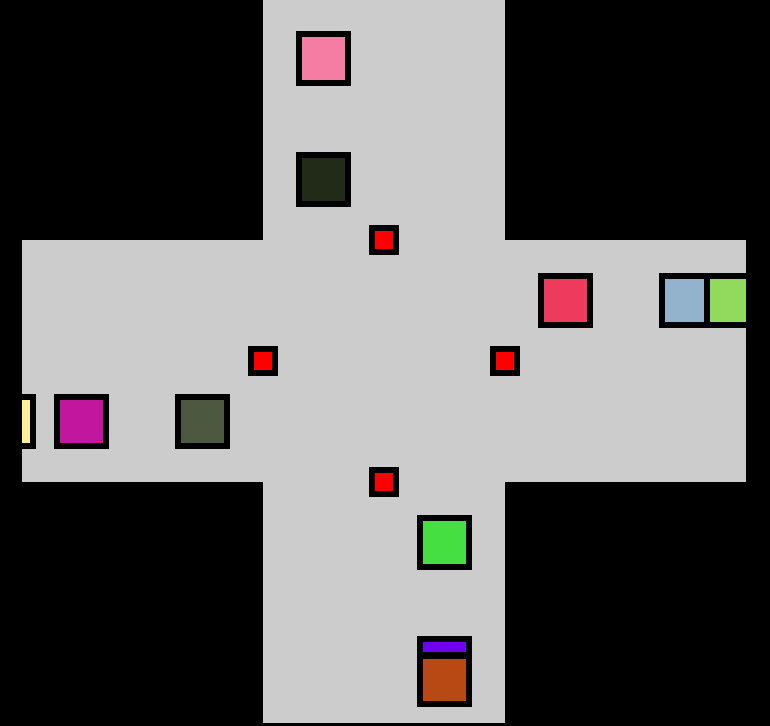
\includegraphics[width=5cm, height=5cm]{sim_intersection}}
\hfill\\
\noindent By placing multiple of these sections next to each other we create something much like a section of city blocks.  Since the user interface to control all stoplights and car destinations would be quite large and a bit daunting to set up, the simulation generates the system randomly.  Each stoplight was set to begin at a random one of its six possible states and have it's \emph{greentime} value set between 5.0 and 15.0 seconds.  The valeus for \emph{yellowtime} and \emph{redtime} were locked at 3.0 and 1.0 seconds respectively.\\\\
Cars are set to randomly enter the system from the edges, with a new car entering every 0.5 seconds.  Moving out of the grid elminates a car from the simulation.

\centerline{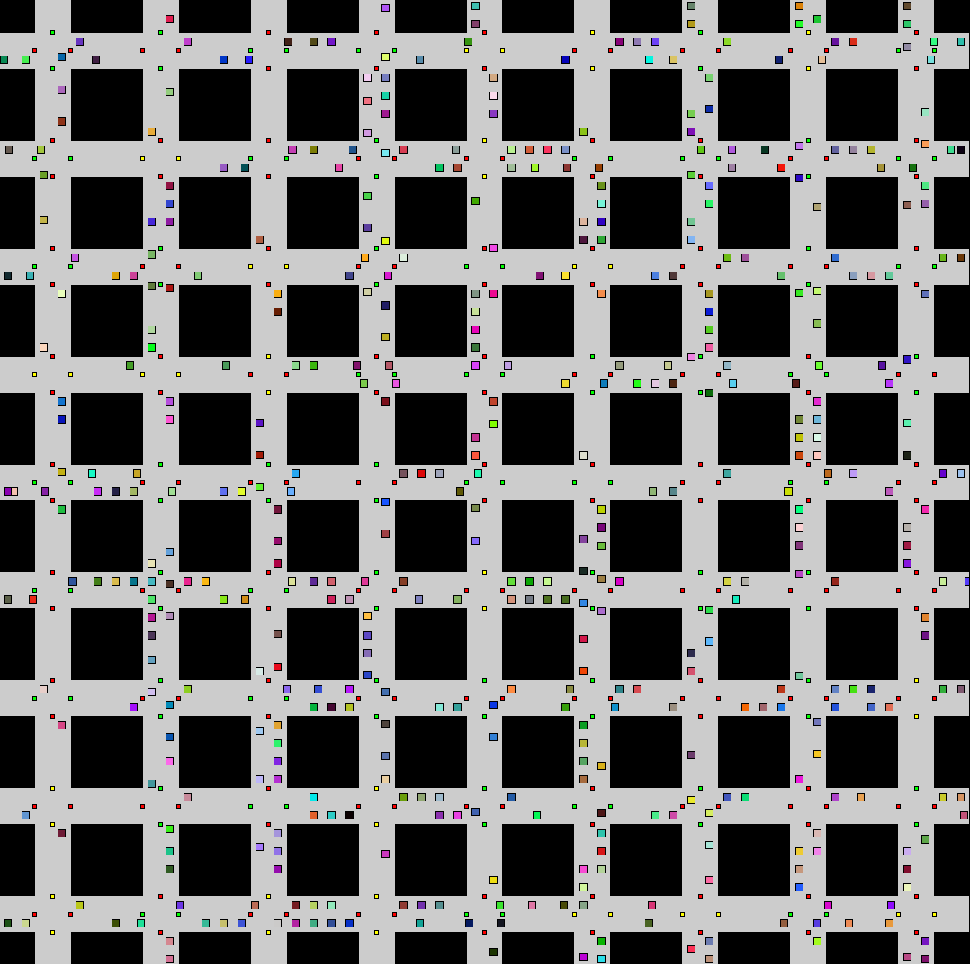
\includegraphics[width=15cm, height=15cm]{full_sim}}

\hfill\\

\section{Conclusions}

The current simulation provides quite a nice representation of city traffic, cars make decisions, don't hit one another and pass through roads and intersections in a realistic way. An interesting observation from the simulation is the fact that while cars only enter from the edges and make decisions randomly, the density of cars remains rather uniform accross the entire simulation. Intersections in the center get clogged just as often as those around the edges.\\\\
Unfortunately, the simulation does not provide the original goal of a sandbox for manipulating and observing conditions.  As a future development, it would be nice to have a user interface for maniuplating all of the variablles in the simulation, as well as a readout of car statistics such as how many lights they hit and the amount of time they stop at lights.  It would also be nice to have an editor system to allow building of custom city layouts, to simulate specific situations.

\pagebreak

\begin{thebibliography}{99}

\bibitem{c1} Nover, H. (2005). Algebraic Cryptanalysis of AES: An Overview. University of Wisconsin, USA.

\end{thebibliography}

\end{document}
